
\section{Runtime Command Interface}
\label{sec:rtcommand_interface}

The Runtime Command Interface allows to connect to a running COMPASS instance and send 
specific commands to it. After command execution, COMPASS will send a reply
containing a command execution status and reply data. This way 
the Runtime Command Interface provides means for interaction with COMPASS from the outside. \\

Starting a COMPASS binary with the '-{}-open\_rt\_cmd\_port' command line option will open the Runtime Command socket
and prepare COMPASS for receiving commands. Then any toolkit or application (Python socket, netcat, etc.)
can be used to connect to this socket at \\

\textbf{IP}: 127.0.0.1 (localhost)

\textbf{Port}: 27960 \\

When connected, s specific command can be sent to the COMPASS client as a string containing the command name and its arguments. \\

\textbf{command\_name} -{}-argument1=VALUE -{}-argument2=VALUE \dots \\

E.g. \textbf{open\_db} -{}-filename="/home/user/PATH\_TO\_FILE" \\

Some commands allow shorter versions without needing to specify the argument names explicitely. \\

\textbf{command\_name} VALUE1 VALUE2 \dots \\

E.g. \textbf{open\_db} "/home/user/PATH\_TO\_FILE" \\

The reply for the issued command will be encoded as JSON string data of the following structure.

\begin{lstlisting}[basicstyle=\small\ttfamily]
{
    "ok": bool                        // Flag indicating if the command could be issued without error 
    "error": string                   // Error string
    "error_additional_info": string   // Additional error information
}
\end{lstlisting}

A second reply will be send after the command has been completed. It takes the following form.

\begin{lstlisting}[basicstyle=\small\ttfamily]
  {
      "ok": bool                        // Flag indicating if the command could be executed without error 
      "error": string                   // Error string
      "error_additional_info": string   // Additional error information 
      "reply": JSON                     // Command reply as JSON object
      "execution_time": string          // Execution time as HH:MM:SS.MSEC
  }
  \end{lstlisting}

The structure of the 'reply' object will depend on the specific command. 

\textbf{Note} that some commands might not send reply data. \\

\textit{Example}: The \textbf{netcat} tool can be used in a terminal to connect to a running COMPASS instance as follows.

\begin{lstlisting}[basicstyle=\small\ttfamily]
> netcat 127.0.0.1 27960
\end{lstlisting}

The netcat tool will then wait for further input. We can for instance open a database externally by typing

\begin{lstlisting}[basicstyle=\small\ttfamily]
> netcat 127.0.0.1 27960
open_db "/home/mcphatty/data/hello_world2.db"
\end{lstlisting}

and pressing ENTER. The reply then looks as follows.

\begin{figure}[H]
  \center
  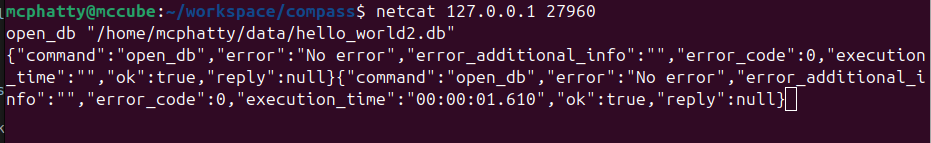
\includegraphics[width=15cm,frame]{figures/netcat_example.png}
%\caption{Example}
\end{figure}

As one can see two JSON objects are send back, the first one 
indicating that the command was successfully issued, the second one that the command 
was successfully executed. As one can also see, the \textbf{open\_db} command does not 
send back reply data, so the 'reply' variable is set to \textit{null}.

\subsection{Runtime Commands}

The existing commands cover various tasks, like creating or opening a database,
importing data into the database, reconstructing reference data, running an evaluation,
retrieving data such as evaluation results, etc. \\

Below is a list of all available commands and their arguments. \\

\textbf{calculate\_artas\_tr\_usage} \\
\textit{associate target reports based on ARTAS usage} \\

\textbf{calculate\_radar\_plot\_positions} \\
\textit{calculate radar plot positions} \\

\textbf{client\_info} \\
\textit{retrieves information about the running compass client} \\

\textbf{close\_db} \\
\textit{closes a currently opened database} \\
strict \dots fail if no database was opened \\

\textbf{create\_db} \\
\textit{creates and opens new database file with given filename, e.g. "/data/file1.db"} \\
filename \dots given filename, e.g. "/data/file1.db" \\

\textbf{evaluate} \\
\textit{run evaluation} \\
run\_filter \dots run evaluation filter before evaluation \\

\textbf{export\_report} \\
\textit{export existing report} \\
report \dots report name, e.g. "EUROCAE ED-87E Evaluation" \\
dir \dots export directory, e.g. "/data/db2/" \\
mode \dots export mode, e.g. "PDF" \\

\textbf{export\_view\_points\_report} \\
\textit{export view points report after with given filename, e.g. "/data/db2/report.tex"} \\
filename \dots given filename, e.g. "/data/db2/report.tex" \\

\textbf{get\_cfg\_data\_sources} \\
\textit{retrieves descriptions of data sources present in the configuration} \\

\textbf{get\_db\_data\_sources} \\
\textit{retrieves descriptions of data sources present in the database} \\

\textbf{get\_dbcontent\_data} \\
\textit{retrieves dbcontent data from the database} \\
dbcontent \dots DBContent to retrieve data for \\
variables \dots variables to retrieve data for \\
utn \dots UTN to retrieve data for \\
max\_size \dots maximum number of results rows \\

\textbf{get\_existing\_reports} \\
\textit{returns a list of names of all existing reports} \\

\textbf{get\_report} \\
\textit{obtain report json data} \\
report \dots name of the report to retrieve, e.g. 'EUROCAE ED-87E Evaluation' \\
section \dots optional ID of the section to retrieve, e.g. 'Report:Results:Overview:Results' \\
See section \nameref{sec:get_report} for more details. \\

\textbf{get\_target} \\
\textit{retrieves a target description for the given UTN} \\
utn \dots UTN of the target to retrieve information for \\

\textbf{get\_target\_stats} \\
\textit{retrieves statistics for the current targets} \\

\textbf{get\_utns} \\
\textit{retrieves UTNS with (optional) target descriptions} \\
nodesc \dots Return a list of existing UTNs without target descriptions \\

\textbf{help} \\
\textit{the help command, generates help information} \\
command \dots command to retrieve help information for \\
details	\dots obtain detailed information such as parameter lists \\

\textbf{import\_asterix\_file} \\
\textit{imports ASTERIX file with given filename, e.g. "/data/file1.ff"} \\
filename \dots given filename, e.g. "/data/file1.json" \\
framing \dots imports ASTERIX file with given  ASTERIX framing, e.g. "none", "ioss", "ioss\_seq", "rff" \\
line \dots imports ASTERIX file with given line e.g. "L2" \\
date \dots imports ASTERIX file with given date, in YYYY-MM-DD format e.g. "2020-04-20" \\
time\_offset \dots imports ASTERIX file with given Time of Day override, in HH:MM:SS.ZZZ" \\
ignore\_time\_jumps \dots ignore 24h time jumps \\

\textbf{import\_asterix\_files} \\
\textit{imports multiple ASTERIX files with given filenames, e.g. '/data/file1.ff;/data/file2.ff'} \\
filenames \dots given filenames, e.g. '/data/file1.ff;/data/file2.ff' \\
framing \dots imports ASTERIX file with given  ASTERIX framing, e.g. "none", "ioss", "ioss\_seq", "rff" \\
line \dots imports ASTERIX file with given line e.g. "L2" \\
date \dots imports ASTERIX file with given date, in YYYY-MM-DD format e.g. "2020-04-20" \\
time\_offset \dots imports ASTERIX file with given Time of Day override, in HH:MM:SS.ZZZ" \\
ignore\_time\_jumps \dots ignore 24h time jumps \\

\textbf{import\_asterix\_network} \\
\textit{imports ASTERIX from defined network UDP streams} \\
time\_offset \dots imports ASTERIX file with given Time of Day override, in HH:MM:SS.ZZZ" \\
max\_lines \dots maximum number of lines per data source during ASTERIX network import, 1..4 \\
ignore\_future\_ts \dots ignore future timestamps \\

\textbf{import\_asterix\_network\_stop} \\
\textit{stops import ASTERIX from network} \\

\textbf{import\_asterix\_pcap\_file} \\
\textit{imports ASTERIX PCAP file with given filename, e.g. '/data/file1.pcap'} \\
filename \dots given filename, e.g. "/data/file1.json" \\
line \dots imports ASTERIX file with given line e.g. "L2" \\
date \dots imports ASTERIX file with given date, in YYYY-MM-DD format e.g. "2020-04-20" \\
time\_offset \dots imports ASTERIX file with given Time of Day override, in HH:MM:SS.ZZZ" \\
ignore\_time\_jumps \dots ignore 24h time jumps \\

\textbf{import\_asterix\_pcap\_files} \\
\textit{imports multiple ASTERIX PCAP files with given filenames, e.g. '/data/file1.pcap;/data/file2.pcap'} \\
filenames \dots given filenames, e.g. '/data/file1.ff;/data/file2.ff' \\
line \dots imports ASTERIX file with given line e.g. "L2" \\
date \dots imports ASTERIX file with given date, in YYYY-MM-DD format e.g. "2020-04-20" \\
time\_offset \dots imports ASTERIX file with given Time of Day override, in HH:MM:SS.ZZZ" \\
ignore\_time\_jumps \dots ignore 24h time jumps \\

\textbf{import\_data\_sources} \\
\textit{imports data sources JSON file with given filename, e.g. '/data/ds1.json'} \\
filename \dots given filename, e.g. "/data/file1.json' \\

\textbf{import\_gps\_trail} \\
\textit{imports gps trail NMEA with given filename, e.g. "/data/file2.txt"} \\
filename \dots given filename, e.g. "/data/file1.nmea' \\
name \dots optional data source name, e.g. "GPS Trail' \\
sac \dots optional sac, e.g. 255 \\
sic \dots optional sic, e.g. 0 \\
tod\_offset \dots optional time of day offset, e.g. -10000.0 \\
date \dots optional override date, e.g. "2025-01-01' \\
mode3a \dots optional mode3a code in octal, e.g.  \\
address \dots optional aircraft address in hex, e.g. "0xffffff' \\
id \dots optional aircraft identification, e.g. "ENTE' \\

\textbf{import\_json} \\
\textit{imports JSON file with given filename, e.g. "/data/file1.json"} \\
filename \dots given filename, e.g. "/data/file1.json" \\

\textbf{import\_sectors\_json} \\
\textit{imports exported sectors JSON with given filename, e.g. "/data/sectors.json"} \\ 
filename \dots given filename, e.g. "/data/file1.json" \\

\textbf{import\_view\_points} \\
\textit{imports view points JSON file with given filename, e.g. '/data/file1.json'} \\
filename \dots given filename, e.g. "/data/file1.json" \\

\textbf{open\_db} \\
\textit{opens existing database file with given filename, e.g. "/data/file1.db"} \\
filename \dots given filename, e.g. "/data/file1.db" \\
assure\_open \dots Only opens the file if it is not already opened \\

\textbf{open\_recent\_db} \\
\textit{opens a database file from the recent file history} \\
filename \dots filename listed in the recent file history, e.g. "file1.db" \\
index \dots index in the recent file history \\

\textbf{quit} \\
\textit{quits the application} \\

\textbf{reconstruct\_references} \\
\textit{reconstruct references} \\
disable\_sensors \dots optional list of sensor names to disables, e.g. "GPS Trail 1;GPS Trail 2' \\

\textbf{set\_data\_sources} \\
\textit{sets data source descriptions} \\
data\_sources \dots Data sources JSON definition \\

\textbf{set\_view\_point} \\
\textit{sets defined view point} \\
view\_point \dots View point JSON definition \\
See section \nameref{sec:appendix_view_points} for how the JSON definition has to be structured. \\

%load_data
%   load data

%get_events
%   retrieves the currently logged events
%      fresh		    return only fresh (unseen) events
%      max_items		maximum number of items to return

%create_db_from_mem
%   creates a database from the current in-memory database

%create_mem_db
%   creates an in-memory database
%      filename	optional future filename of the in-memory database, e.g. "/data/file1.db"

%db_info
%   returns information on the currently opened database
%      help		show command help information

%reconfigure
%   reconfigures the given configurable
%      help		show command help information
%      path		configurable to reconfigure
%      config		json configuration to apply

% uiget
%    retrieves the value of the given ui element
%       help		show command help information
%       object		name of an ui element, object names separated by '.', e.g. 'mainwindow.window1.geographicview1.toolbar'
%       what		which value to retrieve from the ui element (empty = default behavior)
%       json		if present, the result will be returned as a json struct instead of a string
%       visible		if present, the visibility of the ui element will be returned

% uiget_json
%    retrieves the value of the given ui element as json
%       help		show command help information
%       object		name of an ui element, object names separated by '.', e.g. 'mainwindow.window1.geographicview1.toolbar'
%       what		which value to retrieve from the ui element (empty = default behavior)
%       visible		if present, the visibility of the ui element will be returned

% uiinject
%    injects an event into the given ui element
%       help		show command help information
%       object		name of an ui element, object names separated by '.', e.g. 'mainwindow.window1.geographicview1.toolbar'
%       uidelay		delay added after each injected ui event
%       event		event to inject into the ui element

% uirefresh
%    refreshes the given ui element
%       help		show command help information
%       object		name of an ui element, object names separated by '.', e.g. 'mainwindow.window1.geographicview1.toolbar'

% uiset
%    sets an ui element to the given value
%       help		show command help information
%       object		name of an ui element, object names separated by '.', e.g. 'mainwindow.window1.geographicview1.toolbar'
%       uidelay		delay added after each injected ui event
%       value		new value to set, content depending on the addressed ui element


\subsection{Fetching Reports via get\_report}
\label{sec:get_report}

The command \textbf{get\_report} can be used to obtain JSON data of stored reports. \\

Calling it without the -{}-section parameter will fetch a list of all report sections that can be obtained, e.g.

\begin{lstlisting}[basicstyle=\tiny\ttfamily]
{
    "sections" = [          // section id's contained in the report
        "Report:Results",
        "Report:Results:Overview",
        "Report:Results:Sectors",
        "Report:Results:Appendix",
        "Report:Results:Overview:General",
        "Report:Results:Overview:Results",
        "Report:Results:Overview:Targets",
        "Report:Results:Overview:Standard",
        "Report:Results:Sectors:Mandatory DOI",
        "Report:Results:Sectors:Mandatory DOI:Sum",
        "Report:Results:Sectors:Mandatory DOI:Sum:Acceleration Correct",
        "Report:Results:Sectors:Mandatory DOI:Sum:Track Coasting Correct",
        ...
    ]
}
\end{lstlisting}

A specific report section can then be obtained by using the command as follows. \\

\textbf{get\_report} -{}-section=SECTION\_ID \\

This will return the JSON serialized section as documented in section \nameref{sec:report_json_struct},
but the "subsections" variable will not contain the fully serialized subsections,
but only the name and id of each subsection. These can be used to fetch more sections 
via the \textbf{get\_report} command as desired. \\

\textit{Example}: \\

\textbf{get\_report} -{}-section="test Evaluation" "Report:Results:Sectors:Mandatory DOI:Sum" \\

Fetched JSON data: \\

\begin{lstlisting}[basicstyle=\tiny\ttfamily]
{
  "contents": [],
  "id": "Report:Results:Sectors:Mandatory DOI:Sum",
  "name": "Sum",
  "sub_sections": [
      {
        "id": "Report:Results:Sectors:Mandatory DOI:Sum:Acceleration Correct",
        "name": "Acceleration Correct"
      },
      {
        "id": "Report:Results:Sectors:Mandatory DOI:Sum:Track Coasting Correct",
        "name": "Track Coasting Correct"
      },
      {
        "id": "Report:Results:Sectors:Mandatory DOI:Sum:Detection",
        "name": "Detection"
      },
      {
        "id": "Report:Results:Sectors:Mandatory DOI:Sum:Dubious Target",
        "name": "Dubious Target"
      },
      {
        "id": "Report:Results:Sectors:Mandatory DOI:Sum:Dubious Track",
        "name": "Dubious Track"
      },
      ...
  ]
}
\end{lstlisting}

\subsection{Python Example}

The following example will make use of the python class \textit{COMPASSInstance}, 
which makes it quite easy to start a COMPASS instance, connect to it, send commands,
and receive their reply data. \\

For readers interested in obtaining the python code for the COMPASSInstance class and 
more detailed example scripts, please contact us at \href{mailto:compass@openats.at}{compass@openats.at}. \\

Start a COMPASS instance and connect to it:

\begin{lstlisting}[basicstyle=\tiny\ttfamily]

from compass_interface import COMPASSInstance

import json

binary = 'home/user/path_to_binary'

compass_instance = COMPASSInstance() 

ok, error = compass_instance.runCOMPASS(binary = binary,
                                        wait_for_commands = True, # wait until commands can be received
                                        no_cfg_save = True)       # do not save config on close

# handle any errors

# ready to send commands!
\end{lstlisting}

Sending commands:

\begin{lstlisting}[basicstyle=\tiny\ttfamily]

# open database
filename = '/home/user/path_to_db_file'

# escape quotes for filename argument
# the reply variable will hold the command's reply data as a python dictionary
reply, ok, err = compass_instance.interface.sendCommandAndUnpack('open_db \"' + filename + '\"')

# handly any errors 

# get result overview section of existing evaluation report
report_name = 'test Evaluation'
section     = 'Report:Results:Overview:Results'

reply, ok, err = compass_instance.interface.sendCommandAndUnpack('get_report \"{}\" \"{}\"'.format(report_name, section))

# handle any errors 

# the reply will contain the result overview section of the evaluated test standard as a json object
# we can print it to view the reply result
print('Retrieved section:\n')
print(json.dumps(reply, indent = 4))

\end{lstlisting}

Close the COMPASS instance:

\begin{lstlisting}[basicstyle=\tiny\ttfamily]

compass_instance.closeCOMPASS()

\end{lstlisting}

As a result the script will output the retrieved result overview section of a pre-computed Evaluation report.

\begin{figure}[H]
    \hspace*{-2.5cm}
    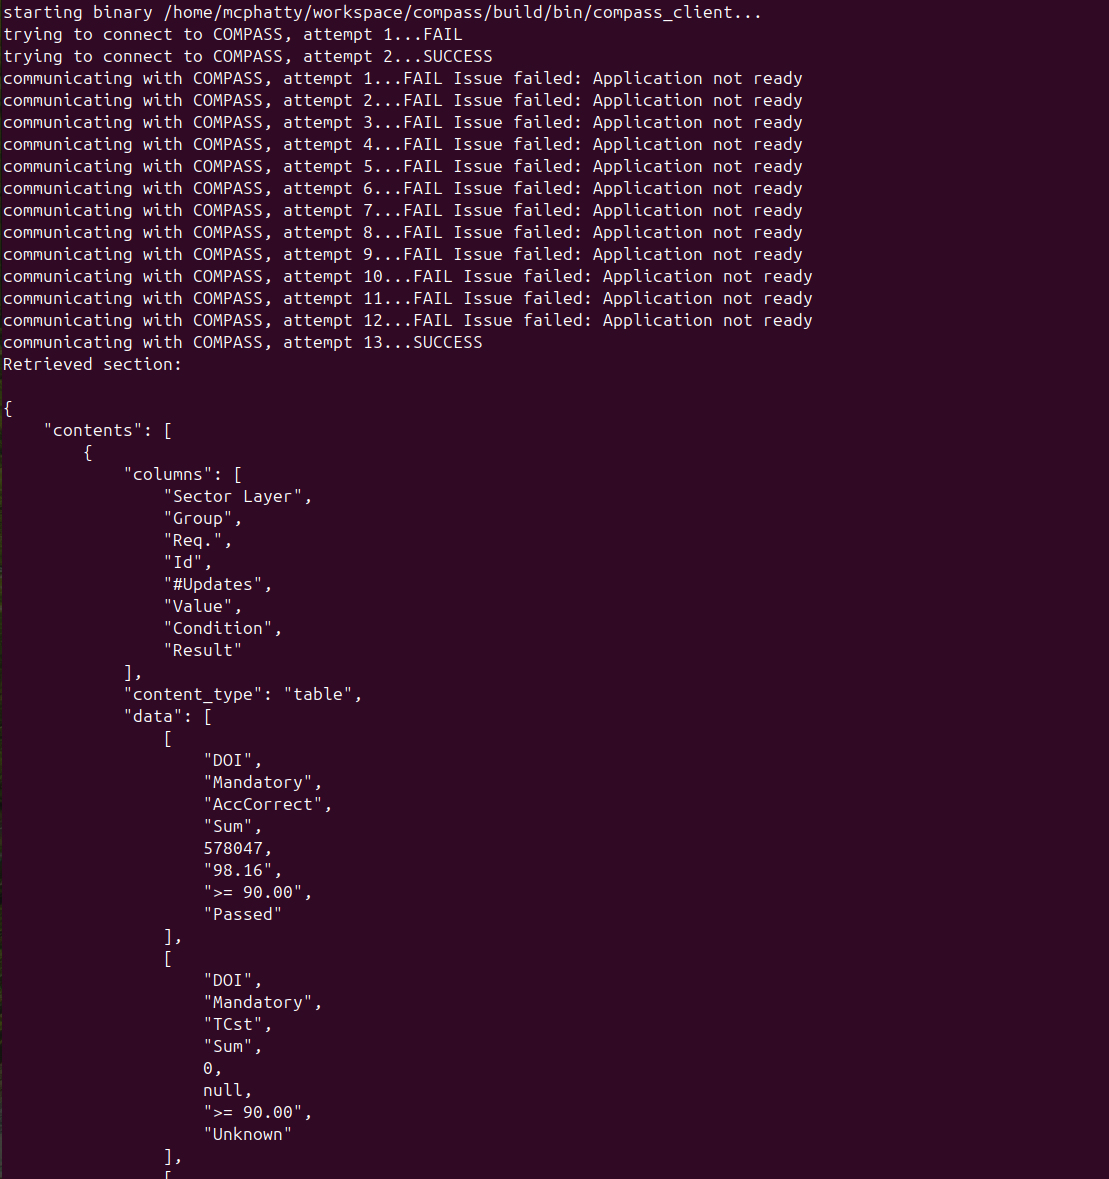
\includegraphics[width=18cm,frame]{figures/script_result.png}
  \caption{Script output}
\end{figure}
